\documentclass[11pt]{article}

\usepackage{enumerate}
\usepackage{amsmath}
\usepackage{color}
\usepackage{listings}
\usepackage{python}
\usepackage{graphicx}
\usepackage{adjustbox}

\graphicspath{{Figures/}}


\newenvironment{equ}{$\hfill\begin{aligned}[t]}{\end{aligned}\hfill \null$}

\lstset{
    tabsize=2
}

\begin{document}

\title{\vspace{-8ex}Stats 330 Assignment 10}
\author{Adam Hammes $\bullet$ hammesa@iastate.edu $\bullet$ Section B}
\maketitle


\section*{Problem 1}

\begin{enumerate}[(a)]
\item
	\begin{tabular}{ r | c | c | c}
		Set & 1 & 2 & 3 \\
		\hline
		Mean & 10.04 & 1.63 & 10.95 \\
		\hline
		Median & 10.10 & 0.98 & 10.93 \\
		\hline
		Stdev & 1.97 & 2.05 & 1.14 \\
		\hline
		1st Quartile & 8.69 & 0.50 & 10.02 \\
		\hline
		3rd Quartile & 11.36 & 1.90 & 11.87
	\end{tabular}

\item \adjustbox{valign=t} {
	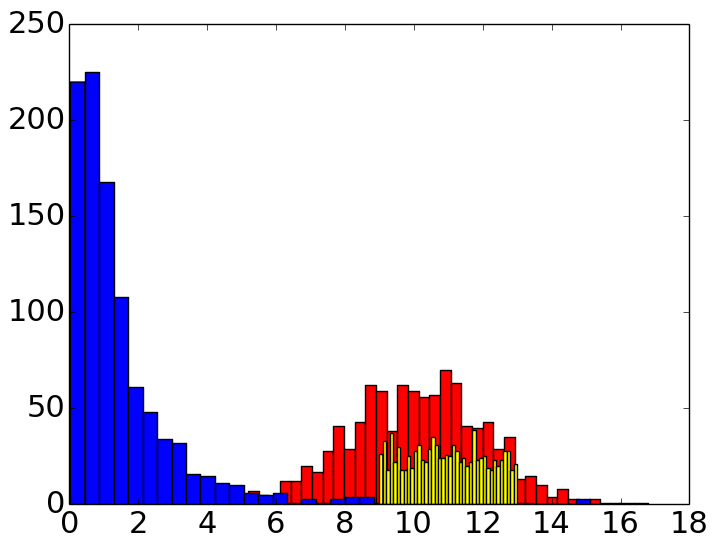
\includegraphics[scale = 0.7]{Histogram.png}
	}

\item \adjustbox{valign=t} {
	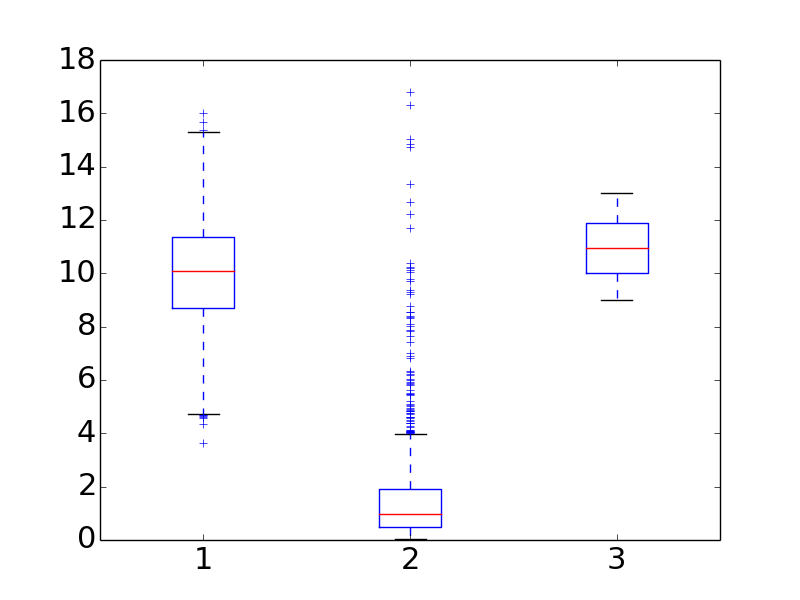
\includegraphics[scale = 0.5]{Boxplot.png}
	}

\end{enumerate}


\section*{Problem 2}

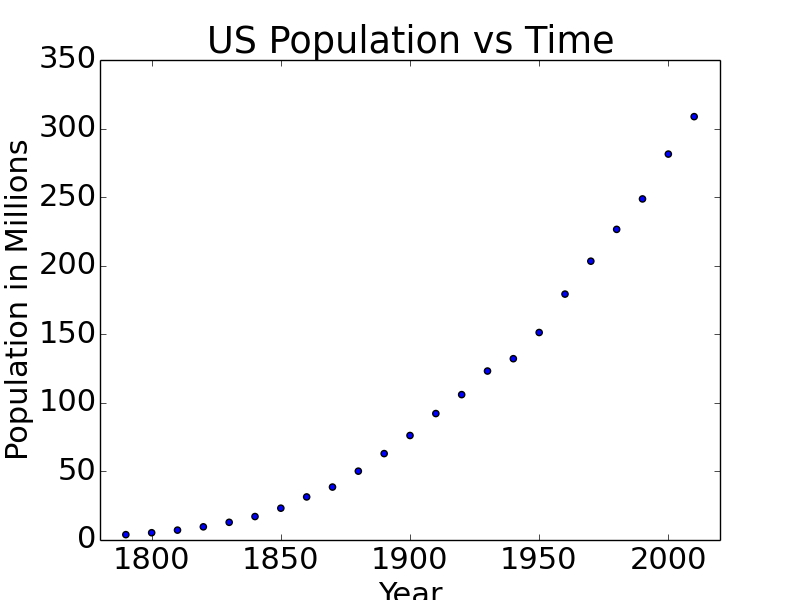
\includegraphics[scale = 0.5]{Figures/Timeplot.png}

The population appears to be going up exponentially. The time plot allows breaks in trends to be spotted easily (such as the small dip around World War II), as well as visually aid in forecasting future trends (I predict that the population will keep increasing).


\section*{Problem 3}

\begin{enumerate}[(a)]
	\item $\lambda$ is the mean of a Poisson distribution, so we can use the first sample moment. $\hat{\lambda} = \bar{X}$

	\item The pmf of Poisson distribution is
	\[P(x) = e^{-\lambda} \dfrac{\lambda^x}{x^!} \]
	whose logarithm is
	\[\text{ln } P(x) = -\lambda + x\, \text{ln } \lambda -  \text{ln}(x!).\]
	Thus we need to maximize
	\begin{align*}
		\text{ln } P(x) &= \sum \limits _{i=1} ^n -\lambda + x\, \text{ln } \lambda -  \text{ln}(x!) \\
		&= -n\lambda + \text{ln } \lambda \sum \limits _{i=1} ^n X_i
	\end{align*}
	Differentiating with respect to $\lambda$ and setting equal to zero yields
	\[\frac{\partial}{\partial x} \text{ln}\ P(x) = -n + \frac{1}{\lambda} \sum \limits _{i=1} ^n X_i = 0 \]
	which has one solution,
	\[ \hat{\lambda} = \frac{1}{n} \sum \limits _{i=1} ^n X_i = \bar{X}. \]

	\item Note that both methods yield the same estimator, $\hat{\lambda} = \bar{X}$. We can therefore estimate $\hat{\lambda}$ as the sample mean, 5.2.


\end{enumerate}



\end{document}